\documentclass[journal,12pt,twocolumn]{IEEEtran}

\usepackage{setspace}
\usepackage{gensymb}

\singlespacing


\usepackage[cmex10]{amsmath}

\usepackage{amsthm}

\usepackage{mathrsfs}
\usepackage{txfonts}
\usepackage{stfloats}
\usepackage{bm}
\usepackage{cite}
\usepackage{cases}
\usepackage{subfig}

\usepackage{longtable}
\usepackage{multirow}

\usepackage{enumitem}
\usepackage{mathtools}
\usepackage{steinmetz}
\usepackage{tikz}
\usepackage{circuitikz}
\usepackage{verbatim}
\usepackage{tfrupee}
\usepackage[breaklinks=true]{hyperref}
\usepackage{graphicx}
\usepackage{tkz-euclide}
\usepackage{float}

\usetikzlibrary{calc,math}
\usepackage{listings}
    \usepackage{color}                                            %%
    \usepackage{array}                                            %%
    \usepackage{longtable}                                        %%
    \usepackage{calc}                                             %%
    \usepackage{multirow}                                         %%
    \usepackage{hhline}                                           %%
    \usepackage{ifthen}                                           %%
    \usepackage{lscape}     
\usepackage{multicol}
\usepackage{chngcntr}

\DeclareMathOperator*{\Res}{Res}

\renewcommand\thesection{\arabic{section}}
\renewcommand\thesubsection{\thesection.\arabic{subsection}}
\renewcommand\thesubsubsection{\thesubsection.\arabic{subsubsection}}

\renewcommand\thesectiondis{\arabic{section}}
\renewcommand\thesubsectiondis{\thesectiondis.\arabic{subsection}}
\renewcommand\thesubsubsectiondis{\thesubsectiondis.\arabic{subsubsection}}


\hyphenation{op-tical net-works semi-conduc-tor}
\def\inputGnumericTable{}                                 %%

\lstset{
%language=C,
frame=single, 
breaklines=true,
columns=fullflexible
}
\begin{document}
\newtheorem{theorem}{Theorem}[section]
\newtheorem{problem}{Problem}
\newtheorem{proposition}{Proposition}[section]
\newtheorem{lemma}{Lemma}[section]
\newtheorem{corollary}[theorem]{Corollary}
\newtheorem{example}{Example}[section]
\newtheorem{definition}[problem]{Definition}

\newcommand{\BEQA}{\begin{eqnarray}}
\newcommand{\EEQA}{\end{eqnarray}}
\newcommand{\define}{\stackrel{\triangle}{=}}
\bibliographystyle{IEEEtran}
\providecommand{\mbf}{\mathbf}
\providecommand{\pr}[1]{\ensuremath{\Pr\left(#1\right)}}
\providecommand{\qfunc}[1]{\ensuremath{Q\left(#1\right)}}
\providecommand{\sbrak}[1]{\ensuremath{{}\left[#1\right]}}
\providecommand{\lsbrak}[1]{\ensuremath{{}\left[#1\right.}}
\providecommand{\rsbrak}[1]{\ensuremath{{}\left.#1\right]}}
\providecommand{\brak}[1]{\ensuremath{\left(#1\right)}}
\providecommand{\lbrak}[1]{\ensuremath{\left(#1\right.}}
\providecommand{\rbrak}[1]{\ensuremath{\left.#1\right)}}
\providecommand{\cbrak}[1]{\ensuremath{\left\{#1\right\}}}
\providecommand{\lcbrak}[1]{\ensuremath{\left\{#1\right.}}
\providecommand{\rcbrak}[1]{\ensuremath{\left.#1\right\}}}
\theoremstyle{remark}
\newtheorem{rem}{Remark}
\newcommand{\sgn}{\mathop{\mathrm{sgn}}}
\providecommand{\abs}[1]{\vert#1\vert}
\providecommand{\res}[1]{\Res\displaylimits_{#1}} 
\providecommand{\norm}[1]{\lVert#1\rVert}
%\providecommand{\norm}[1]{\lVert#1\rVert}
\providecommand{\mtx}[1]{\mathbf{#1}}
\providecommand{\mean}[1]{E[ #1 ]}
\providecommand{\fourier}{\overset{\mathcal{F}}{ \rightleftharpoons}}
%\providecommand{\hilbert}{\overset{\mathcal{H}}{ \rightleftharpoons}}
\providecommand{\system}{\overset{\mathcal{H}}{ \longleftrightarrow}}
	%\newcommand{\solution}[2]{\textbf{Solution:}{#1}}
\newcommand{\solution}{\noindent \textbf{Solution: }}
\newcommand{\cosec}{\,\text{cosec}\,}
\providecommand{\dec}[2]{\ensuremath{\overset{#1}{\underset{#2}{\gtrless}}}}
\newcommand{\myvec}[1]{\ensuremath{\begin{pmatrix}#1\end{pmatrix}}}
\newcommand{\mydet}[1]{\ensuremath{\begin{vmatrix}#1\end{vmatrix}}}
\numberwithin{equation}{subsection}
\makeatletter
\@addtoreset{figure}{problem}
\makeatother
\let\StandardTheFigure\thefigure
\let\vec\mathbf
\renewcommand{\thefigure}{\theproblem}
\def\putbox#1#2#3{\makebox[0in][l]{\makebox[#1][l]{}\raisebox{\baselineskip}[0in][0in]{\raisebox{#2}[0in][0in]{#3}}}}
     \def\rightbox#1{\makebox[0in][r]{#1}}
     \def\centbox#1{\makebox[0in]{#1}}
     \def\topbox#1{\raisebox{-\baselineskip}[0in][0in]{#1}}
     \def\midbox#1{\raisebox{-0.5\baselineskip}[0in][0in]{#1}}
\vspace{3cm}
\title{ASSIGNMENT 3}
\author{Ananthoju Pranav Sai \\ AI20BTECH11004}
\maketitle
\newpage
\bigskip
\renewcommand{\thefigure}{\theenumi}
\renewcommand{\thetable}{\theenumi}
Download all python codes from 
\begin{lstlisting}
https://github.com/Ananthoju-Pranav-Sai/EE3900/blob/main/Assignment-3/codes/Assignment-3.py
\end{lstlisting}
%
and latex-tikz codes from 
%
\begin{lstlisting}
https://github.com/Ananthoju-Pranav-Sai/EE3900/tree/main/Assignment-3/Assignment-3.tex
\end{lstlisting}
%
\section{Construction 2.11}
Construct PLAN where PL = 4, LA = 6.5, $\angle$P = 90$^\circ$,$\angle$A = 110$^\circ$ and $\angle$N = 85$^\circ$,
%
\section{Solution}
\begin{lemma}
    Let ABCD be a quadrilateral with 
    \begin{align}
        \norm{B-A} = a\\
        \norm{C-B} = b\\
        \angle A = \theta\\
        \angle C = \beta\\
        \angle D = \gamma\\
        \vec{A} = \myvec{0\\
                         0}\\
        \vec{B} = \myvec{a\\
                         0}   
    \end{align}
    then the remaining vectors can be found using 
    \begin{align}
        \vec{C} = \vec{B}+b\myvec{\cos{(180-\alpha)}\\
                                  \sin{(180-\alpha)}}
    \end{align}
    where $\alpha$ = $360-(\theta+\beta+\gamma)$
    \begin{align}
        \vec{D} = d\myvec{\cos{\theta}\\
                          \sin{\theta}}
    \end{align}
    where 
    \begin{align}
        d &= \norm{A-D} = e\times\brak{\frac{\sin{\brak{\beta-\sin^{-1}\brak{{\frac{a\sin\alpha}{e}}}}}}{\sin\gamma}}\\
        e &= \norm{C-A} = \sqrt{a^2+b^2-2ab\cos{\alpha}}
    \end{align}
\end{lemma}
\begin{proof}
    Let,
    \begin{align}
        \angle {ACB} = \beta_1\\
        \angle {ACD} = \beta_2\\
        \implies \beta_1 + \beta_2 = \beta \label{a}
    \end{align}
    Now in $\triangle$ ABC applying cosine rule gives,
    \begin{align}
        e &= \sqrt{a^2+b^2-2ab\cos{\alpha}}
    \end{align}
    and in $\triangle$ ABC applying sine rule gives,
    \begin{align}
        \frac{\sin{\angle{ACB}}}{AB} = \frac{\sin B}{AC}\\
        \implies \frac{\sin{\beta_1}}{a} = \frac{\sin{\alpha}}{e}\\
        \implies \beta_1 = \sin^{-1}\brak{\frac{a\sin\alpha}{e}}   \label{b}     
    \end{align}
    and in $\triangle$ ACD applying sine rule gives,
    \begin{align}
        \frac{\sin{\angle{ACD}}}{AD} = \frac{\sin D}{AC}\\
        \implies \frac{\sin{\beta_2}}{d} = \frac{\sin{\gamma}}{e}\\
        \implies d = e\times\brak{\frac{\sin{\brak{\beta-\sin^{-1}\brak{{\frac{a\sin\alpha}{e}}}}}}{\sin\gamma}}
    \end{align}
\end{proof}
Given, 
\begin{align}
    \angle P &= 90^\circ = \theta\\
    \angle A &= 110^\circ = \beta\\
    \angle N &= 85^\circ = \gamma\\
    \implies \angle L &= 75^\circ = \alpha\\
    \norm{\vec{L}-\vec{P}} &= 4 = a\\
    \norm{\vec{A}-\vec{L}} &= 6.5 = b\\
    &\vec{P} = \myvec{0\\
                     0}\\
    &\vec{L} = \myvec{4\\
                      0}
\end{align}
Let,
\begin{align}
    &\theta = \angle L\\
    &\norm{\vec{A}-\vec{N}} = c\\
    &\norm{\vec{N}-\vec{P}} = d\\
    &\norm{\vec{A}-\vec{P}} = e
\end{align}
We know that,
\begin{align}
        d &= e\times\brak{\frac{\sin{\brak{\beta-\sin^{-1}\brak{{\frac{a\sin\alpha}{e}}}}}}{\sin\gamma}}\label{c}\\
        e &= \sqrt{a^2+b^2-2ab\cos{\alpha}}\\
        \implies e &= 6.7\label{d}
\end{align}
using $\eqref{d}$ in $\eqref{c}$ we get
\begin{align}
    d=6.49
\end{align}
then for $\vec{A}$ we have,
\begin{align}
    \vec{A} &= \vec{L}+b\myvec{\cos{(180-\alpha)}\\
                              \sin{(180-\alpha)}}\\
    \implies \vec{A} &= \myvec{4\\
                              0}+6.5\myvec{\cos{105}\\
                                            \sin{105}}\\
    \implies \vec{A} &= \myvec{2.318\\
                              6.279}
\end{align}
and for $\vec{N}$ we have,
\begin{align}
    \vec{N} &= d\myvec{\cos{\theta}\\
                       \sin{\theta}}\\
    \implies \vec{N} &= \myvec{0\\
                               6.49}
\end{align}
\begin{figure}[!ht]
    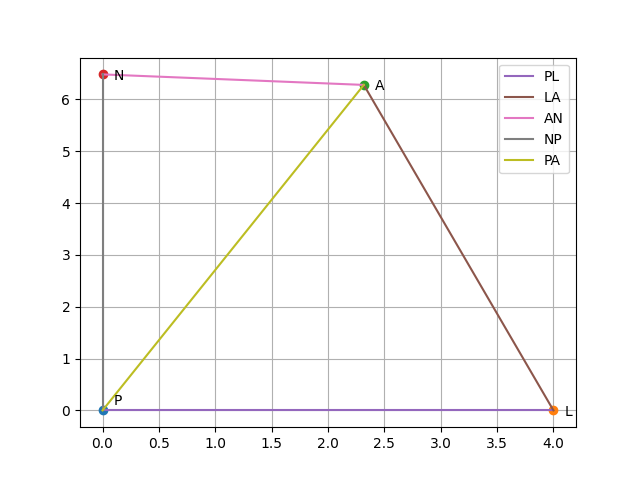
\includegraphics[ width=\columnwidth, height=6 cm]{Quadrilateral_PLAN.png}
    \caption{Quadrilateral PLAN}
    \label{fig:Quadrilateral PLAN}	
\end{figure}
\end{document}
